\documentclass{article}
\usepackage[margin=2.5cm, top=4cm, headheight=25pt]{geometry}
\usepackage{amsmath, amssymb, enumitem, fancyhdr, graphicx}
\usepackage[indent=20pt]{parskip}
\usepackage[hidelinks]{hyperref}
\usepackage{xcolor}
\usepackage{listings}
\usepackage{subcaption}
\usepackage{url}
\usepackage[most]{tcolorbox}
\usepackage{lastpage}
\usepackage{tikz}
\usetikzlibrary{arrows.meta}
\tcbuselibrary{listingsutf8} % Support for lstlistings within tcolorbox

\newtcolorbox[auto counter, number within=section]{question}[1][]{%
    colframe=gray!80,                      % Dark gray frame
    colback=gray!5,                       % Light gray background
    coltitle=black,                        % Black title
    title=\textbf{Question~\thetcbcounter}, % Bold title
    fonttitle=\bfseries\large,             % Subtle title font size
    rounded corners,                   % Slightly more rounded corners
    boxrule=0.25mm,                         % Thinner border for a sleek look
    enhanced,                              % Enhanced box features
    attach boxed title to top left={xshift=2mm, yshift=-2mm},
    boxed title style={colframe=gray!80, colback=gray!5, boxrule=0.25mm},
    % Title styling
    #1
}

\bibliographystyle{IEEEtran}
\graphicspath{{./images/}}

% -- Custom Variables --
\def\me{Rajdeep Gill 7934493}
\def\course{ECE 3760}
\def\labsection{A01}

\def\labno{6}
\def\title{Assignment 6: Garage Security System}

% -- Styling for code snippets --
\lstset{
    basicstyle=\ttfamily\scriptsize,           % Basic font style
    keywordstyle=\color{blue},            % Keywords color
    commentstyle=\color{gray},            % Comments color
    stringstyle=\color{teal},             % Strings color
    numbers=left,                         % Line numbers on the left
    numberstyle=\tiny\color{gray},        % Line number style
    stepnumber=1,                         % Line number step
    numbersep=10pt,                       % Space between line numbers and code
    backgroundcolor=\color{lightgray!10}, % Background color
    frame=single,                         % Adds a frame around the code
    breaklines=true,                      % Line breaking for long lines
    captionpos=b,                         % Caption position
    showspaces=false,                     % Don't show spaces
    showstringspaces=false                % Don't show spaces in strings
}
\renewcommand{\lstlistingname}{Code Snippet}

\renewcommand{\arraystretch}{1.2} % For less-ugly tables
\setlength\parindent{0pt}

%----- Samples 
% Questions:
%   \begin{question}[title=Custom Question Title]
%       Question details
%   \end{question}

% Tables:
%   \begin{table}[htbp]
%       \centering
%       \caption{Table Caption}
%       \begin{tabular}{ll}
%           \toprule
%           \textbf{Column 1} & \textbf{Column 2} \\
%           \midrule
%           Row 1 & Row 2 \\
%           Row 3 & Row 4 \\
%           \bottomrule
%       \end{tabular}
%   \end{table} 

% Figures:
%   Single figure:
%       \begin{figure}[htbp]
%           \centering
%           \includegraphics[width=0.5\textwidth]{example-image}
%           \caption{Figure Caption}
%       \end{figure}
%   Multiple figures:
%       \begin{figure}[htbp]
%           \centering
%           \begin{subfigure}[b]{0.5\textwidth}
%               \includegraphics[width=\textwidth]{example-image-a}
%               \caption{First subfigure}
%           \end{subfigure}
%           \begin{subfigure}[b]{0.5\textwidth}
%               \includegraphics[width=\textwidth]{example-image-b}
%               \caption{Second subfigure}
%           \end{subfigure}
%           \caption{Main figure}
%       \end{figure}

\begin{document}

% --------------------------------------------------------------------------------
% TITLE
% --------------------------------------------------------------------------------

\begin{center}
    \huge \title

    \vspace{2mm}
    \hrule

    \vspace{4mm}
    \large \me

    \vspace{2mm}
    \large \course~\labsection

    \vspace{2mm}
    \today
\end{center}

\vspace{4mm}

% --------------------------------------------------------------------------------
% END TITLE
% --------------------------------------------------------------------------------

\newpage


\vspace{1cm}
\newpage

\pagestyle{fancy}
\fancyhead[L]{\large Assignment \labno}
\fancyhead[R]{\large \me}

\fancyfoot[C]{Page \thepage~of~\pageref{LastPage}}

% --------------------------------------------------------------------------------
% BODY
% --------------------------------------------------------------------------------
\section{Security System Desgin}

To design a successful security system, we need to consider the following requirements and constraints:
\begin{itemize}
    \item System should work in an industrial/residential environment
    \item Powered by 120V AC
    \item Ability to arm and disarm via a coded switch, or a keyed system
    \item Monitor two doors
\end{itemize}

With these requirements, a simple flow chart can be created to outline the system's operation. This flow chart is shown in \autoref{fig:flowchart}.

\begin{figure}[ht!]
    \centering
    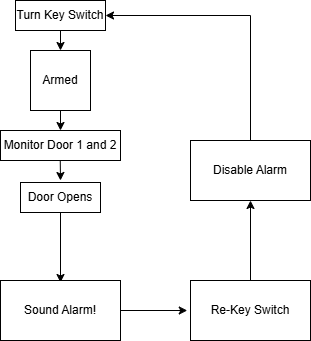
\includegraphics[width=0.3\textwidth]{flowchart1.png}
    \caption{Flow chart for the security system}
    \label{fig:flowchart}
\end{figure}

The system is armed by turning the key switch to the on position. This will arm the system and begin monitoring the two doors. If either door is opened, the alarm will sound and can be silenced by using the key to turn the switch to the off position. 

The ladder logic for this system is shown in \autoref{fig:ladder}. It mimics what was described above. The two normally closed switches, when open will allow power to flow to the alarm, sounding it if the key switch is in the on position.

\begin{figure}[ht!]
    \centering
    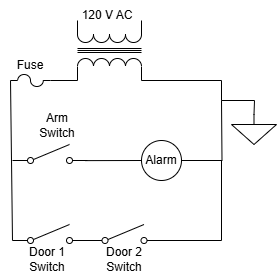
\includegraphics[width=0.3\textwidth]{ladder.png}
    \caption{Ladder logic for the security system}
    \label{fig:ladder}
\end{figure}

Further iterating on this design, we can use the inplace coded switch to arm and disarm the system instead of a keyed switch. A timer can also be added to the system to allow for a delay between the door being opened and the alarm sounding. This is shown in \autoref{fig:flowchart2}.

\begin{figure}[ht!]
    \centering
    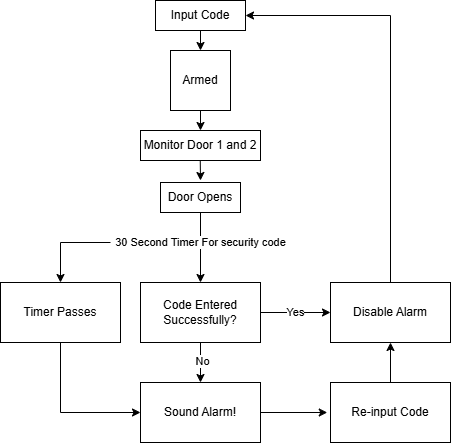
\includegraphics[width=0.3\textwidth]{flowchart2.png}
    \caption{Flow chart for the security system with coded switch and timer}
    \label{fig:flowchart2}
\end{figure}

A programmable logic controller (PLC) can be used to implement this system. The PLC will take in inputs from the coded switch and the two door switches. The PLC will then output to the alarm based on the states of the inputs and a timer. This would ensure a more rugged and reliable system than a relay-based system.

% --------------------------------------------------------------------------------
% END BODY
% --------------------------------------------------------------------------------

\end{document}
